
\chapter{Kalkulus Numerik\label{chap:Numerical-Calculus}}

\section{\label{sec:NumericalRudiments}Dasar-Dasar Kalkulus Numerik}

\subsection{Gagasan dasar}

$g(x)=x-\frac{2\pi}{3}\sin(x)$ memiliki akar di antara $0$ dan $\pi$.
Anda sedang mencoba berbagai metode dan mulai tertarik pada bagaimana
pemilihan nilai awal memengaruhi hasilnya. Dengan menggunakan metode
Newton, Anda menyelidiki bagaimana pemilihan $x_{0}$ memengaruhi
$x_{2}$. Anda menjalankan beberapa pengujian dan memperoleh data
berikut.

\begin{center}
\begin{tabular}{c|c}
$x_{0}$ & $x_{2}$\tabularnewline
\hline 
$93/70$ & $2.084603181618954$\tabularnewline
$95/70$ & $2.055494116570853$\tabularnewline
$97/70$ & $2.030278824314539$\tabularnewline
$99/70$ & $2.009751835391139$\tabularnewline
$101/70$ & $1.993574976724822$\tabularnewline
$103/70$ & $1.981091507449763$\tabularnewline
$105/70$ & $1.971614474758557$\tabularnewline
\end{tabular}
\par\end{center}

\noindent Dengan menggunakan iterasi titik tetap pada $f(x)=\frac{2\pi}{3}\sin(x)$,
Anda memutuskan untuk menelaah bagaimana pemilihan $x_{0}$ memengaruhi
$x_{10}$, bukan $x_{2}$ karena iterasi titik tetap pada umumnya
lambat konvergen. Anda menjalankan beberapa pengujian atas metode
ini dan memperoleh data berikut.

\begin{center}
\begin{tabular}{c|c}
$x_{0}$ & $x_{10}$\tabularnewline
\hline 
$1/7$ & $1.949880891899200$\tabularnewline
$2/7$ & $1.951091775564697$\tabularnewline
$3/7$ & $1.923339403354019$\tabularnewline
$4/7$ & $1.941460911122824$\tabularnewline
$5/7$ & $1.960870620285721$\tabularnewline
$6/7$ & $1.965674866641883$\tabularnewline
$1$ & $1.961228252911260$\tabularnewline
\end{tabular}
\par\end{center}

Dalam eksperimen dengan metode Newton, $x_{2}$ merupakan fungsi dari
$x_{0}$, sedangkan dalam eksperimen iterasi titik tetap, $x_{10}$
merupakan fungsi dari $x_{0}$. Jadi, Anda mulai memandang keduanya
sepenuhnya terlepas dari persoalan pencarian akar semula. Dalam bentuk
tabelnya, keduanya hanyalah dua fungsi yang beberapa nilainya kita
ketahui, tetapi selebihnya tidak banyak. Seperti apakah bentuk fungsi-fungsi
ini? Apakah informasi yang kita miliki cukup untuk menemukan turunannya,
dan dengan demikian ekstrem lokalnya? Dapatkah kita menemukan antiturunannya?
Inilah pokok bahasan kalkulus numerik. Kita tentu dapat menghampiri
semua itu. 

Dalam bab \ref{chap:Interpolation} kita telah mempelajari cara menghampiri
fungsi dengan interpolasi, sehingga kita tahu bahwa data tabel dapat
digunakan untuk menghampiri fungsi itu sendiri. Namun, bagaimana dengan
turunan dan integralnya? Polinom mudah diturunkan dan diintegralkan.
Barangkali kita dapat menggunakan turunan dan integral polinom interpolasi
untuk menghampiri turunan dan integral $x_{2}(x_{0})$ dan $x_{10}(x_{0})$.
Ternyata memang bisa! 

Untuk menghindari kebingungan akibat penggunaan $x_{0}$ untuk beberapa
tujuan, fungsi-fungsi tersebut akan kita namai ulang sebagai $\nu(x)$
untuk $x_{2}(x_{0})$ dan $\varphi(x)$ untuk $x_{10}(x_{0})$. Dengan
demikian, kita memperoleh $\nu(93/70)=2.0846\ldots$, $\nu(95/70)=2.0554\ldots$,
dan seterusnya. Demikian pula, kini kita memperoleh $\varphi(1/7)=1.9498\ldots$,
$\varphi(2/7)=1.9510\ldots$, dan seterusnya. Kita juga akan membiasakan
diri menyebut koordinat-$x$ dari titik-titik interpolasi yang ditentukan
sebagai simpul.\index{simpul} Dengan demikian, simpul yang kita miliki
untuk $\nu$ adalah $93/70$, $95/70$, dan seterusnya. Simpul yang
kita miliki untuk $\varphi$ adalah $1/7$, $2/7$, dan seterusnya.

\noindent\begin{digression}{$\nu$ dan $\varphi$} 

\noindent$\nu$ adalah huruf ketiga belas (dalam bentuk huruf kecil)
dalam alfabet Yunani dan dilafalkan \texttt{nu}. $\varphi$ adalah
huruf kedua puluh satu (dalam bentuk huruf kecil) dalam alfabet Yunani
dan dilafalkan \texttt{fi}. Huruf \texttt{fi} juga ditulis sebagai
$\phi$, tetapi dalam matematika jauh lebih umum dijumpai bentuk varian
$\varphi$, mungkin untuk menghindari kerancuan antara \texttt{fi}
dan himpunan kosong, $\emptyset$. Bentuk huruf kapital dari $\nu$
dan $\varphi$ adalah $N$ dan $\Phi$, secara berturut-turut.

\noindent\end{digression}

Kita mulai dengan meninjau polinom interpolasi pada tiga simpul. Untuk
$\nu$, kita menggunakan simpul $93/70$, $99/70$, dan $1.5$, lalu
memperoleh
\[
P_{2,\nu}(x)=.07673215587088045x^{2}\text{\textminus}.07445530457646088x+1.95895140161684.
\]
Untuk $\varphi$, kita menggunakan simpul $1/7$, $4/7$, dan $1$,
lalu memperoleh
\[
P_{2,\varphi}(x)=2.498590686342254x^{2}-7.726543017101505x+7.939599956140455.
\]
Kita telah menambahkan subskrip kedua pada $P_{2}$ untuk membedakan
polinom interpolasi bagi $\nu$ dari polinom bagi $\varphi$. Kini
kita dapat menghampiri turunan dan integral dari $\nu$ dan $\varphi$
dengan menggunakan $P_{2,\nu}$ dan $P_{2,\varphi}$, secara berturut-turut:
\begin{eqnarray*}
\nu'(x) & \approx & P_{2,\nu}'(x)=4.997181372684508x-7.726543017101505\\
\varphi'(x) & \approx & P_{2,\varphi}'(x)=.1534643117417609x-.07445530457646088\\
\int\nu\,dx & \approx & \int P_{2,\nu}dx=.8328635621140847x^{3}-3.863271508550753x^{2}+7.939599956140455x+C\\
\int\varphi\,dx & \approx & \int P_{2,\varphi}dx=.02557738529029348x^{3}-.03722765228823044x^{2}+1.95895140161684x+D.
\end{eqnarray*}
Jadi, sebagai contoh,
\begin{eqnarray*}
\nu'(1.4) & \approx & P_{2,\nu}'(1.4)\\
 & = & 4.997181372684508(1.4)-7.726543017101505\\
 & = & -.7304890953431942\\
\varphi'(0.5) & \approx & P_{2,\varphi}'(0.5)\\
 & = & .1534643117417609(0.5)-.07445530457646088\\
 & = & .002276851294419568
\end{eqnarray*}
 dan 
\begin{eqnarray*}
\int_{1.4}^{1.5}\nu(x)dx & \approx & \int_{1.4}^{1.5}P_{2,\nu}(x)dx\\
 & = & \left[.8328635621140847x^{3}-3.863271508550753x^{2}+7.939599956140455x\right]_{1.4}^{1.5}\\
 & = & .1991481658283149\\
\int_{0}^{1}\varphi(x)dx & \approx & \int_{0}^{1}P_{2,\varphi}(x)dx\\
 & = & \left[.02557738529029348x^{3}-.03722765228823044x^{2}+1.95895140161684x\right]_{0}^{1}\\
 & = & 1.947301134618903.
\end{eqnarray*}

\noindent Selesai! Latihan ini merangkum seluruh strategi. Jika diberikan
beberapa nilai dari suatu fungsi yang selebihnya tidak diketahui,
kita akan menghampiri fungsi yang tidak diketahui itu dengan sebuah
polinom. Selanjutnya, kita akan menghampiri turunan dan integral fungsi
yang tidak diketahui dengan menurunkan dan mengintegralkan polinom
tersebut. Tidak banyak lagi yang perlu dikatakan tentang gagasan ini.
Namun, masih banyak yang perlu dibahas tentang otomasi, akurasi, dan
efisiensi, yang menjadi fokus sisa bab ini. Akan tetapi, sebelum menangani
persoalan tersebut, kita akan meninjau kembali $\nu$ dan $\varphi$.

Dengan menggunakan seluruh simpul $\nu$, dan dengan bantuan sistem
aljabar komputer, kita menghitung polinom interpolasi berderajat enam\label{integrationWithP6}
\begin{eqnarray*}
P_{6,\nu}(x) & = & -1342.393417879939x^{6}+11632.43754466623x^{5}-41996.4789301455x^{4}\\
 &  & +80851.91317212582x^{3}-87536.60487741232x^{2}+50528.3026241064x\\
 &  & -12144.27629915625.
\end{eqnarray*}
Dengan menggunakan seluruh simpul $\varphi$ (serta sistem aljabar
komputer), kita menghitung polinom interpolasi berderajat enam
\begin{eqnarray*}
P_{6,\varphi}(x) & = & -25.41848741926543x^{6}+97.00017832506126x^{5}-147.1805326076494x^{4}\\
 &  & +111.7996194440324x^{3}-43.71110414341027x^{2}+8.049781257197147x\\
 &  & +1.421773396945804.
\end{eqnarray*}
Sekali lagi, kita menambahkan subskrip kedua untuk membedakan polinom
interpolasi bagi $\nu$ dari polinom bagi $\varphi$. Kini kita dapat
memperoleh taksiran kedua untuk $\nu'(1.4)$, $\varphi'(0.6)$, $\int_{1.4}^{1.5}\nu\,dx$,
dan $\int_{0}^{1}\varphi\:dx$:
\begin{eqnarray*}
\nu'(1.4) & \approx & P_{6,\nu}'(1.4)\approx-.7178145479410887\\
\varphi'(0.5) & \approx & P_{6,\varphi}'(0.5)\approx.1729311759579151\\
\int_{1.4}^{1.5}\nu(x)dx & \approx & \int_{1.4}^{1.5}P_{6,\nu}(x)dx\approx.1991932206801721\\
\int_{0}^{1}\varphi(x)dx & \approx & \int_{0}^{1}P_{6,\varphi}(x)dx\approx1.925578216262883.
\end{eqnarray*}
Tabel \ref{tab:numericalCalcFirstStab} merangkum delapan taksiran
yang telah kita buat sejauh ini. 
\begin{table}
\hrule \caption{\label{tab:numericalCalcFirstStab}Penaksiran turunan dan integral
$\nu$ dan $\varphi$.}

\centering{}\medskip{}
\begin{tabular}{c|cc}
besaran & menggunakan $P_{2}$ & menggunakan $P_{6}$\tabularnewline
\hline 
$\nu'(1.4)$ & $-.7304890953431942$  & $-.7178145479410887$\tabularnewline
$\varphi'(0.5)$ & $.002276851294419568$  & $.1447147284558277$\tabularnewline
$\int_{1.4}^{1.5}\nu(x)dx$ & $.1991481658283149$ & $.1991932206801721$\tabularnewline
$\int_{0}^{1}\varphi(x)dx$ & $1.947301134618903$ & $1.925578216262883$\tabularnewline
\end{tabular}\medskip{}
\hrule 
\end{table}
Empat digit pertama pada taksiran $\int_{1.4}^{1.5}\nu(x)dx$ sama,
dan dua digit pertama pada taksiran $\int_{0}^{1}\varphi(x)dx$ sama.
Jadi, ada kesesuaian tertentu di antara taksiran integral tersebut.
Namun, taksiran turunannya tidak begitu selaras. Taksiran untuk $\nu'(1.4)$
hanya sama pada digit signifikan pertamanya. Keduanya menunjukkan
$\nu'(1.4)\approx-.7$. Namun, pada dasarnya tidak ada kesesuaian
antara taksiran $\varphi'(0.5)$. Salah satu hampiran bernilai lebih
dari 60 kali hampiran lainnya! Berdasarkan analisis sederhana ini,
kita akan sulit memercayai salah satu dari kedua taksiran $\varphi'(0.5)$.
Kita pun sebaiknya hanya memercayai beberapa digit pertama taksiran
lainnya. Kelak akan kita lihat bahwa perbandingan semacam ini dapat
digunakan agar komputer menentukan apakah suatu hampiran baik atau
tidak.

\subsection{Permasalahan}

Ada tiga permasalahan pada metode penaksiran turunan dan integral
yang baru saja diuraikan.
\begin{enumerate}
\item \textbf{Efisiensi.} Demi keperluan ilustrasi dan untuk memahami konsep
dasar kalkulus numerik, ada baiknya kita menghitung beberapa polinom
interpolasi seperti yang dilakukan pada subbagian sebelumnya. Namun,
cara tersebut rumit dan memakan waktu. Kita akan mencurahkan banyak
upaya untuk menemukan jalan pintas bagi metode langsung ini agar lebih
efisien dan praktis.
\item \textbf{Otomasi.} Metode numerik dimaksudkan untuk dijalankan oleh
komputer, bukan oleh manusia dengan kalkulator. Kita perlu menemukan
cara agar komputer dapat menangani polinom interpolasi. Permasalahan
ini berkaitan erat dengan efisiensi. Bagaimanapun, suatu algoritma
akan efisien jika dapat dieksekusi dengan cepat oleh komputer!
\item \textbf{Akurasi.} Sejauh ini, hampir tidak ada yang kita lakukan untuk
menentukan seberapa akurat hampiran kita. Kita perlu memahami suku
galat dengan lebih baik agar mengetahui cara menggunakan metode ini
secara akurat.
\end{enumerate}
Sekarang, kita mulai mengatasi ketiga permasalahan ini, tetapi sebagian
besar pembahasannya kita sisakan untuk bagian-bagian berikutnya.

Dalam bab \ref{chap:Interpolation}, kita memberi label pada simpul-simpul
suatu fungsi interpolasi sebagai $x_{0},x_{1},\ldots,x_{n}$. Akan
bermanfaat jika kita mulai menyebutnya $x_{0}+\theta_{0}h,x_{0}+\theta_{1}h,\ldots,x_{0}+\theta_{n}h$
sebagai gantinya. Untuk sebagian besar analisis, kita akan menggunakan
$x_{0}+\theta h$ alih-alih $x$ untuk titik tempat kita menginginkan
suatu taksiran. Substitusi ini dapat disebut perubahan variabel atau
kalibrasi ulang sumbu-$x$.

Untuk melihat bagaimana hal ini membantu analisis, tinjaulah polinom
interpolasi berderajat paling tinggi 2 untuk $f$ dengan simpul 
\[
x_{0}+\theta_{0}h,\ x_{0}+\theta_{1}h,\mbox{ dan }x_{0}+\theta_{2}h.
\]
Dalam notasi pada bab \ref{chap:Interpolation}, kita memperoleh 
\[
P_{2}(x)=\frac{(x-x_{1})(x-x_{2})}{(x_{0}-x_{1})(x_{0}-x_{2})}f(x_{0})+\frac{(x-x_{0})(x-x_{2})}{(x_{1}-x_{0})(x_{1}-x_{2})}f(x_{1})+\frac{(x-x_{0})(x-x_{1})}{(x_{2}-x_{0})(x_{2}-x_{1})}f(x_{2}),
\]
 tetapi dengan notasi baru, kita mengganti $x_{0}$ dengan $x_{0}+\theta_{0}h$,
$x_{1}$ dengan $x_{0}+\theta_{1}h$, $x_{2}$ dengan $x_{0}+\theta_{2}h$,
dan $x$ dengan $x_{0}+\theta h$, sehingga diperoleh
\begin{eqnarray}
P_{2}(x_{0}+\theta h) & = & \frac{(\theta-\theta_{1})(\theta-\theta_{2})}{(\theta_{0}-\theta_{1})(\theta_{0}-\theta_{2})}f(x_{0}+\theta_{0}h)\nonumber \\
 &  & +\frac{(\theta-\theta_{0})(\theta-\theta_{2})}{(\theta_{1}-\theta_{0})(\theta_{1}-\theta_{2})}f(x_{0}+\theta_{1}h)\nonumber \\
 &  & +\frac{(\theta-\theta_{0})(\theta-\theta_{1})}{(\theta_{2}-\theta_{0})(\theta_{2}-\theta_{1})}f(x_{0}+\theta_{2}h).\label{eq:p2relative}
\end{eqnarray}
Pada dasarnya, kita hanya menukar $x$ dengan $\theta$ dan $x_{i}$
dengan $\theta_{i}$. Perubahan yang tampak sepele ini sebenarnya
merupakan langkah maju yang sangat besar! Rumus ini memperlihatkan
bahwa nilai sebenarnya dari $x_{i}$ tidaklah penting. Yang penting
hanyalah letaknya relatif terhadap suatu titik acuan, $x_{0}$, yang
diukur dalam satuan panjang karakteristik $h$. $\theta$ dan $\theta_{i}$
merupakan ukuran tersebut. Pada hakikatnya, hal ini menjadikan $x_{0}$
sebagai titik asal dan $h$ sebagai satuan ukur pada sumbu-$x$. Kita
mengukur semua nilai dengan menghitung berapa kelipatan $h$ jaraknya
dari $x_{0}$.

Untuk menggambarkan manfaatnya, andaikan kita memiliki tiga simpul
yang berjarak sama, sehingga simpul terkecil dan terbesar berjarak
sama dari simpul ketiga, yaitu simpul tengah. Dengan menetapkan simpul
tengah sebagai titik acuan, $x_{0}$, dan panjang karakteristik, $h$,
sebagai jarak dari simpul tengah ini ke simpul lainnya, kita kemudian
dapat melabelinya sebagai
\[
x_{0}-h,\ x_{0},\mbox{ dan }x_{0}+h.
\]
Kita pun telah sampai pada hal pokok. Tidak menjadi masalah apakah
himpunan simpulnya adalah $\{1,2,3\}$ atau $\{80,90,100\}$ atau
$\{-4.3,-4.2,-4.1\}$. Dalam setiap himpunan tersebut, terdapat tiga
simpul, dan salah satunya merupakan titik tengah dari dua simpul lainnya.
Setiap himpunan simpul sama dengan himpunan $\{x_{0}-h,x_{0},x_{0}+h\}$
untuk nilai tertentu dari $x_{0}$ dan $h$. Dengan demikian, jika
kita dapat melakukan suatu analisis dengan himpunan $\{x_{0}-h,x_{0},x_{0}+h\}$,
kita memperoleh informasi tentang cara bekerja dengan himpunan simpul
mana pun, seperti $\{1,2,3\}$ atau $\{80,90,100\}$ atau $\{-4.3,-4.2,-4.1\}$
dan seterusnya. 

Kembali ke himpunan simpul $\{x_{0}-h,x_{0},x_{0}+h\}$. Untuk himpunan
simpul ini, kita memperoleh $\theta_{0}=-1$, $\theta_{1}=0$, dan
$\theta_{2}=1$. Dengan menyubstitusikannya ke \ref{eq:p2relative},
\begin{eqnarray*}
P_{2}(x_{0}+\theta h) & = & \frac{(\theta)(\theta-1)}{(-1)(-2)}f(x_{0}-h)+\frac{(\theta+1)(\theta-1)}{(1)(-1)}f(x_{0})+\frac{(\theta+1)(\theta)}{(2)(1)}f(x_{0}+h)\\
 & = & \frac{\theta^{2}-\theta}{2}f(x_{0}-h)+(1-\theta^{2})f(x_{0})+\frac{\theta^{2}+\theta}{2}f(x_{0}+h).
\end{eqnarray*}
Kini rumus ini dapat digunakan untuk memperoleh parabola interpolasi
pada sembarang himpunan tiga simpul yang berjarak sama. 

Untuk mencoba menerapkan rumus ini pada $\nu$, tinjaulah simpul $93/70$,
$99/70$, dan $105/70$. Karena $\frac{99}{70}-\frac{93}{70}=\frac{105}{70}-\frac{99}{70}$,
kita memiliki himpunan simpul berbentuk $\{x_{0}-h,x_{0},x_{0}+h\}$
dengan $x_{0}=\frac{99}{70}$ dan $h=\frac{6}{70}=\frac{3}{35}$.
Kebetulan $1.4=\frac{99}{70}-\frac{1}{6}\cdot\frac{3}{35}$, sehingga
kita menggunakan $\theta=-\frac{1}{6}$ untuk menghitung $P_{2,\nu}(1.4)$:
\begin{eqnarray*}
P_{2,\nu}(1.4) & = & P_{2,\nu}\left(x_{0}-\frac{1}{6}h\right)\\
 & = & \frac{\left(-\frac{1}{6}\right)^{2}+\frac{1}{6}}{2}\nu\left(\frac{93}{70}\right)+\left(1-\left(-\frac{1}{6}\right)^{2}\right)\nu\left(\frac{99}{70}\right)+\frac{\left(-\frac{1}{6}\right)^{2}-\frac{1}{6}}{2}\nu\left(\frac{105}{70}\right)\\
 & = & \frac{7\nu\left(\frac{93}{70}\right)+70\nu\left(\frac{99}{70}\right)-5\nu\left(\frac{105}{70}\right)}{72}\\
 & = & \frac{7(2.084603181618954)+70(2.009751835391139)-5(1.971614474758557)}{72}\\
 & = & 2.019677477429439.
\end{eqnarray*}
Taksiran ini tampak cukup baik karena nilainya berada di antara $\nu(93/70)\approx2.085$
dan $\nu(99/70)\approx2.009$ tetapi jauh lebih dekat ke $2.009$.
Bagaimanapun, $1.4$ berada di antara $93/70\approx1.328$ dan $99/70\approx1.414$
tetapi jauh lebih dekat ke $1.414$. Persamaan \ref{eq:lagrangeInterpolatingPolynomialError}
memberi kita gambaran tentang tingkat ketelitian yang dapat diharapkan
dari taksiran ini.

Namun, mari kita mundur beberapa langkah dalam perhitungan ini. Konstanta-konstanta
pada langkah $\frac{7\nu\left(\frac{93}{70}\right)+70\nu\left(\frac{99}{70}\right)-5\nu\left(\frac{105}{70}\right)}{72}$
ditentukan semata-mata dari nilai $\theta$ dan $\theta_{i}$. Sementara
itu, $\frac{93}{70}$, $\frac{99}{70}$, dan $\frac{105}{70}$ hanyalah
ketiga simpul, yaitu $x_{0}-h,x_{0},x_{0}+h$, sehingga yang sebenarnya
kita miliki di sini adalah suatu kaidah, atau rumus, untuk nilai $P_{2}(x_{0}-\frac{1}{6}h)$
bagi \textit{setiap} polinom interpolasi berderajat paling tinggi
2 pada simpul $x_{0}-h$, $x_{0}$, dan $x_{0}+h$:
\[
\nu\left(x_{0}-\frac{1}{6}h\right)\approx P_{2,\nu}\left(x_{0}-\frac{1}{6}h\right)=\frac{7\nu(x_{0}-h)+70\nu(x_{0})-5\nu(x_{0}+h)}{72}.
\]
Tidak ada pula yang istimewa pada fungsi $\nu$ yang digunakan dalam
rumus ini. Tidak satu pun dari konstanta $-\frac{1}{6}$, $7$, $70$,
$-5$, maupun $72$ bergantung pada $\nu$, melainkan hanya pada jarak
antarsimpul. Oleh karena itu, untuk sebarang fungsi $f$, dari perhitungan
ini kita dapat memperoleh rumus hampiran ringkas
\begin{equation}
f\left(x_{0}-\frac{1}{6}h\right)\approx\frac{7f(x_{0}-h)+70f(x_{0})-5f(x_{0}+h)}{72}.\label{eq:p2formula}
\end{equation}

\noindent Rumus ini menunjukkan tujuan sebenarnya dari menyatakan
ulang nilai $x_{i}$ dalam bentuk $x_{0}$, $h$, dan $\theta_{i}$.
Dengan cara ini, kita memperoleh rumus yang berlaku bagi seluruh kelas
simpul, bukan hanya satu himpunan simpul tertentu.

Untuk $\varphi$, simpul $\frac{1}{7}$, $\frac{4}{7}$, dan $1$
berjarak sama, sehingga himpunan $\{\frac{1}{7},\frac{4}{7},1\}$
memiliki bentuk $\{x_{0}-h,x_{0},x_{0}+h\}$ dengan $x_{0}=\frac{4}{7}$
dan $h=\frac{3}{7}$. Bukan suatu kebetulan bahwa $\frac{4}{7}-\frac{1}{6}\cdot\frac{3}{7}=0.5$,
sehingga $\varphi(0.5)=\varphi(x_{0}-\frac{1}{6}h)$ dengan $x_{0}=\frac{4}{7}$
dan $h=\frac{3}{7}$. Kini kita dapat menggunakan rumus \ref{eq:p2formula}
untuk menghampiri $\varphi(0.5)$!
\begin{eqnarray*}
\varphi(0.5) & \approx & P_{2,\varphi}(0.5)=\frac{7\varphi(x_{0}-h)+70\varphi(x_{0})-5\varphi(x_{0}+h)}{72}\\
 & = & \frac{7(1.9498808918992)+70(1.941460911122824)-5(1.96122825291126)}{72}\\
 & = & 1.94090678829633.
\end{eqnarray*}
Kali ini, kita sepenuhnya menghindari perhitungan dan evaluasi langsung
terhadap $P_{2,\varphi}$. Rumus \ref{eq:p2formula} memungkinkan
kita menghitung $P_{2,\varphi}(0.5)$ secara langsung dari nilai $\varphi$
pada ketiga simpul. Tidak perlu menghitung, merujuk kembali, mengevaluasi,
atau menyederhanakan $P_{2,\varphi}$! Semua itu telah dilakukan dalam
penurunan rumus. Sangat cepat. Sangat efisien.

\subsection{Stensil\index{stensil}}

Rumus seperti \ref{eq:p2formula} hanya berlaku untuk sekumpulan simpul
dan titik evaluasi yang memiliki geometri (posisi relatif) yang sama
dengan geometri yang digunakan untuk menurunkan rumus tersebut. Oleh
karena itu, kita perlu mencatat geometri yang digunakan untuk menurunkan
rumus-rumus semacam itu. Untuk keperluan tersebut, kita sering menyebut
sekumpulan simpul tertentu beserta titik evaluasinya sebagai stensil.
Sebagai contoh, simpul-simpul $x_{0}-h$, $x_{0}$, $x_{0}+h$ dengan
titik evaluasi $x_{0}-\frac{1}{6}h$ membentuk sebuah stensil---susunan
relatif titik-titik yang dapat diskalakan (dengan mengubah nilai $h$)
dan ditranslasikan (dengan mengubah nilai $x_{0}$). Pada garis bilangan,
stensil ini tampak seperti

\begin{center}
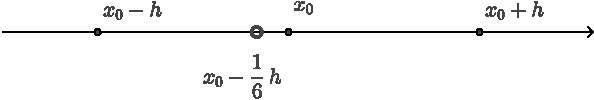
\includegraphics{figures/calculus-rudiments01}.
\par\end{center}

\noindent$x_{0}$ dapat berada di mana saja dan $h$ dapat bernilai
berapa pun, bahkan negatif. Fleksibilitas inilah yang membuat rumus
seperti \ref{eq:p2formula} berguna.

Sekarang, misalkan data yang kita miliki tidak berjarak sama, tetapi
kita tertarik pada sebuah titik di tengah-tengah dua titik lainnya.
Stensil tiga titik yang sesuai akan menggunakan simpul-simpul $x_{0}-h$,
yaitu simpul paling kiri, $x_{0}+h$, yaitu simpul paling kanan, dan
$x_{0}+\theta_{1}h$ untuk suatu $\theta_{1}$ di antara $-1$ dan
$1$, yaitu simpul tengah, dengan titik evaluasi $x_{0}$, yaitu titik
di tengah-tengah simpul paling kiri dan paling kanan. Untuk $\theta_{1}=\frac{1}{3}$,
stensil ini tampak seperti

\begin{center}
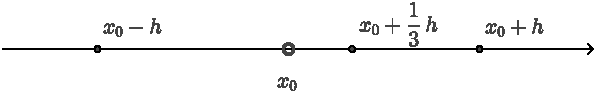
\includegraphics{figures/calculus-rudiments02}.
\par\end{center}

\noindent Kita juga dapat menurunkan rumus untuk $P_{2}(x_{0})$ berdasarkan
nilai $f$ pada ketiga simpul tersebut. Dengan menyubstitusikan $\theta=0$,
$\theta_{0}=-1$, $\theta_{1}=\frac{1}{3}$, dan $\theta_{2}=1$ ke
dalam persamaan \ref{eq:p2relative}, kita memperoleh
\begin{eqnarray*}
P_{2}(x_{0}) & = & \frac{(-\frac{1}{3})(-1)}{(-\frac{4}{3})(-2)}f(x_{0}-h)+\frac{(1)(-1)}{(\frac{4}{3})(-\frac{2}{3})}f(x_{0}+\frac{1}{3}h)+\frac{(1)(-\frac{1}{3})}{(2)(\frac{2}{3})}f(x_{0}+h)\\
 & = & \frac{f(x_{0}-h)+9f(x_{0}+\frac{1}{3}h)-2f(x_{0}+h)}{8},
\end{eqnarray*}
sekali lagi, sebuah rumus ringkas yang berlaku untuk fungsi $f$.
Tidak perlu menghitung polinom interpolasi atau mengevaluasinya secara
langsung untuk setiap data yang sesuai dengan stensil ini. Bagian
tersebut sudah dihitung dan disederhanakan.

\subsection{Turunan\label{subsec:Derivatives}\index{diferensiasi numerik}}

Rumus untuk turunan dapat diperoleh dengan cara yang sama. Setelah
diturunkan untuk suatu stensil, rumus tersebut dapat digunakan dengan
sangat mudah dan efisien untuk data lain yang sesuai dengan stensil
yang sama. Sekarang kita akan mencari rumus untuk turunan pertama,
$P_{2}'(x_{0}-\frac{1}{6}h)$, pada stensil

\begin{center}
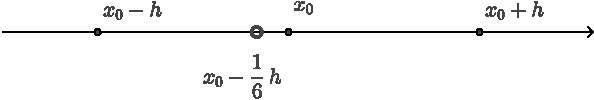
\includegraphics{figures/calculus-rudiments01}
\par\end{center}

\noindent yang digunakan sebelumnya. Kita mulai dengan mengamati bahwa
dalam \ref{eq:p2relative} $x$ merupakan fungsi dari $\theta$. Secara
khusus, $x(\theta)=x_{0}+h\theta$, sehingga $\frac{d}{d\theta}x(\theta)=h$.
Berdasarkan aturan rantai, $\frac{d}{d\theta}P_{2}(\theta)=\frac{d}{dx}P_{2}(x)\cdot\frac{d}{d\theta}x(\theta)=h\frac{d}{dx}P_{2}(x)$.
Dari persamaan \ref{eq:p2relative}, kita kemudian memperoleh 
\begin{eqnarray}
\frac{d}{dx}P_{2}(x) & = & \frac{\frac{d}{d\theta}P_{2}(\theta)}{h}\nonumber \\
 & = & \frac{(\theta-\theta_{1})+(\theta-\theta_{2})}{h(\theta_{0}-\theta_{1})(\theta_{0}-\theta_{2})}f(x_{0}+\theta_{0}h)\nonumber \\
 &  & +\frac{(\theta-\theta_{0})+(\theta-\theta_{2})}{h(\theta_{1}-\theta_{0})(\theta_{1}-\theta_{2})}f(x_{0}+\theta_{1}h)\nonumber \\
 &  & +\frac{(\theta-\theta_{0})+(\theta-\theta_{1})}{h(\theta_{2}-\theta_{0})(\theta_{2}-\theta_{1})}f(x_{0}+\theta_{2}h).\label{eq:p2relativeDerivative}
\end{eqnarray}
Secara khusus, ketika $\theta_{0}=-1$, $\theta_{1}=0$, $\theta_{2}=1$,
dan $\theta=-\frac{1}{6}$, kita memperoleh
\begin{eqnarray}
P_{2}'\left(x_{0}-\frac{1}{6}h\right) & = & \frac{-\frac{1}{6}-\frac{7}{6}}{h(-1)(-2)}f(x_{0}-h)+\frac{\frac{5}{6}-\frac{7}{6}}{h(1)(-1)}f(x_{0})+\frac{\frac{5}{6}-\frac{1}{6}}{h(2)(1)}f(x_{0}+h)\label{eq:derivativeDumb}\\
 & = & \frac{-2f(x_{0}-h)+f(x_{0})+f(x_{0}+h)}{3h}.\nonumber 
\end{eqnarray}
Kini kita memiliki rumus untuk $P_{2}'(x_{0}-\frac{1}{6}h)\approx f'(x_{0}-\frac{1}{6}h)$
pada stensil dengan simpul-simpul $x_{0}-h$, $x_{0}$, $x_{0}+h$
dan $x=x_{0}-\frac{1}{6}h$. Rumus ini sekarang dapat kita gunakan
untuk mengaproksimasi $\nu'(1.4)$ dan $\varphi'(0.5)$.
\begin{eqnarray*}
\nu'(1.4) & \approx & \frac{-2\nu(\frac{93}{70})+\nu(\frac{99}{70})+\nu(\frac{105}{70})}{3(\frac{3}{35})}\\
 & = & \frac{-2(2.084603181618954)+2.009751835391139+1.971614474758557)}{9/35}\\
 & = & -.7304890953430477.
\end{eqnarray*}
Perhatikan bahwa hasil ini tidak persis sama dengan yang kita peroleh
dalam tabel \ref{tab:numericalCalcFirstStab} untuk $\nu'(1.4)$ dengan
menggunakan $P_{2}$. Kedua taksiran tersebut berbeda pada beberapa
digit terakhir. Hal ini disebabkan oleh galat titik-mengambang yang
memengaruhi perhitungan dengan cara yang berbeda. Secara umum, perhitungan
langsung dari polinom interpolasi menghasilkan galat yang lebih besar
karena data diproses jauh lebih intensif. Namun, sebaiknya jangan
memercayai beberapa digit terakhir dalam kedua perhitungan. Selanjutnya,
\begin{eqnarray*}
\varphi'(0.5) & \approx & \frac{-2\varphi(\frac{1}{7})+\varphi(\frac{4}{7})+\varphi(1)}{3(\frac{3}{7})}\\
 & = & \frac{-2(1.9498808918992)+1.941460911122824+1.96122825291126)}{9/7}\\
 & = & .002276851294420679.
\end{eqnarray*}
Sekali lagi, hasil ini mendekati aproksimasi dalam tabel \ref{tab:numericalCalcFirstStab},
tetapi tidak persis sama karena galat titik-mengambang yang berbeda
dalam kedua perhitungan tersebut. Namun, inti pembahasannya sudah
jelas. Menggunakan rumus berbasis stensil lebih baik daripada bekerja
langsung dengan polinom interpolasi. Cara ini lebih mudah, lebih efisien,
dan dapat diotomatisasi.

Sebelum beralih ke integrasi, ada satu hal lagi yang perlu diperhatikan.
Ketika mencoba mengaproksimasi $f$ dengan polinom interpolasi, tidak
banyak gunanya mempertimbangkan stensil seperti

\begin{center}
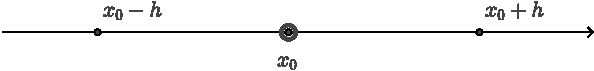
\includegraphics{figures/calculus-rudiments03},
\par\end{center}

\noindent yang titik evaluasinya merupakan salah satu simpul. Berdasarkan
definisi $P_{n}$, kita tahu bahwa $P_{n}(x_{i})=f(x_{i})$ untuk
setiap simpul $x_{i}$. Oleh karena itu, ``rumus'' tersebut adalah
$f(x_{i})=P_{2}(x_{i})$, dan rumus itu bersifat eksak, bukan aproksimasi.
Rumus ini juga tidak terlalu informatif karena fakta tersebut merupakan
salah satu dasar yang kita gunakan untuk menghitung $P_{2}$! Di sisi
lain, stensil semacam itu memang masuk akal ketika mencoba mengaproksimasi
turunan $f$. Tidak ada jaminan bahwa turunan $P_{n}$ akan sama dengan
turunan $f$ di titik mana pun, bahkan di simpul-simpulnya. Dengan
menyubstitusikan $\theta_{0}=-1$, $\theta_{1}=0$, $\theta_{2}=1$,
dan $\theta=0$ ke \ref{eq:p2relativeDerivative}, kita memperoleh
\begin{eqnarray}
P_{2}'(x_{0}) & = & \frac{1}{h(-1)(-2)}f(x_{0}-h)+\frac{1+(-1)}{h(1)(-1)}f(x_{0})+\frac{1}{h(2)(1)}f(x_{0}+h)\nonumber \\
 & = & \frac{f(x_{0}+h)-f(x_{0}-h)}{2h},\label{eq:centeredDifferenceNaive}
\end{eqnarray}
sebagai contoh.

\subsection{Integral\index{integrasi numerik}\index{integrasi numerik|seealso{kuadratur}}}

Untuk rumus integrasi, kita menggunakan stensil yang dimodifikasi.
Kita memerlukan simpul-simpul beserta ujung-ujung interval integrasi,
yang akan ditandai dengan tanda kurung siku: $[$ untuk ujung kiri
dan $]$ untuk ujung kanan. Namun, prosesnya serupa. Kita mencari
rumus untuk polinom interpolasi dan, alih-alih mengintegralkan fungsi
yang tidak diketahui, kita mengintegralkan polinom interpolasi.

Dengan mengikuti prosedur ini, kita dapat menurunkan rumus integral
untuk $f$ pada stensil 

\begin{center}
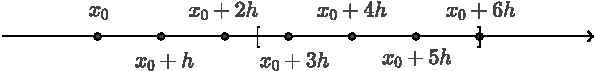
\includegraphics{figures/calculus-rudiments04},
\par\end{center}

\noindent sebagai contoh. Langkah-langkah aljabarnya sederhana tetapi
panjang, sehingga tidak kami tampilkan di sini. Sebaiknya gunakan
sistem aljabar komputer untuk menurunkan rumus semacam ini. Hasilnya,
yaitu aproksimasi integral pada $[x_{0}+2.5h,x_{0}+6h]$ dengan menggunakan
simpul-simpul $x_{0}$, $x_{0}+h$, $x_{0}+2h$, $x_{0}+3h$, $x_{0}+4h$,
$x_{0}+5h$, dan $x_{0}+6h$, adalah
\begin{eqnarray*}
\int_{x_{0}+2.5h}^{x_{0}+6h}f(x)dx & \approx & \frac{h}{138240}\left[42056f(x_{0}+6h)+201831f(x_{0}+5h)+63357f(x_{0}+4h)\right.\\
 &  & \left.+195902f(x_{0}+3h)-28518f(x_{0}+2h)+10731f(x_{0}+h)-1519f(x_{0})\right].
\end{eqnarray*}
Rumus ini kini dapat digunakan untuk mengaproksimasi $\int_{1.4}^{1.5}\nu(x)dx$
sebagai pengganti pengintegralan polinom interpolasi secara langsung
seperti yang dilakukan \vpageref{integrationWithP6}. Silakan substitusikan
nilai-nilai $\nu$ yang sesuai, lalu bandingkan jawaban Anda dengan
jawaban pada tabel \vpageref{tab:numericalCalcFirstStab}. Jawaban
\vpageref{ans:integralFormula1}.

Stensil untuk aproksimasi $\int_{0}^{1}\varphi(x)dx$ menggunakan
$P_{6,\varphi}$ tampak seperti 

\begin{center}
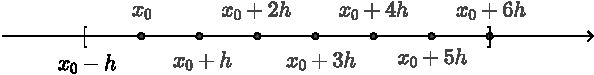
\includegraphics{figures/calculus-rudiments05},
\par\end{center}

\noindent yang berbeda dari stensil yang kita gunakan untuk mengaproksimasi
$\int_{1.4}^{1.5}\nu(x)dx$. Oleh karena itu, rumus aproksimasinya
juga berbeda. Kita memerlukan rumus integral pada $[x_{0}-h,x_{0}+6h]$
dengan simpul-simpul $x_{0}$, $x_{0}+h$, $x_{0}+2h$, $x_{0}+3h$,
$x_{0}+4h$, $x_{0}+5h$, dan $x_{0}+6h$. Simpul-simpulnya sama seperti
sebelumnya, tetapi interval integrasinya berbeda. Hasilnya adalah
\begin{eqnarray}
\int_{x_{0}-h}^{x_{0}+6h}f(x)dx & \approx & \frac{h}{8640}\left[5257f(x_{0}+6h)-5880f(x_{0}+5h)+59829f(x_{0}+4h)\right.\nonumber \\
 &  & \left.-81536f(x_{0}+3h)+102459f(x_{0}+2h)-50568f(x_{0}+h)+30919f(x_{0})\right].\label{eq:integral7dumb}
\end{eqnarray}
Sekali lagi, rumus semacam ini sebaiknya diturunkan dengan menggunakan
sistem aljabar komputer. Silakan substitusikan nilai-nilai $\varphi$
yang sesuai untuk mengaproksimasi $\int_{0}^{1}\varphi(x)dx$ dan
bandingkan hasil Anda dengan hasil pada tabel \vpageref{tab:numericalCalcFirstStab}.
Jawaban \vpageref{ans:integralFormula2}.

\subsection{Konsep Kunci}
\begin{description}
\item [{simpul:}] \index{simpul}absis (koordinat pertama) suatu titik
data yang digunakan dalam interpolasi.
\item [{aproksimasi~polinomial:}] \index{aproksimasi polinomial}mengaproksimasi
nilai suatu fungsi, turunannya, atau integralnya berdasarkan nilai
yang bersesuaian dari suatu polinom interpolasi.
\item [{stensil:}] \index{stensil}susunan relatif absis yang digunakan
dalam aproksimasi polinomial.
\end{description}
\noindent\startexercises 

\subsection{Latihan}
\begin{enumerate}
\item Buatlah sketsa stensil yang sesuai dengan rumus tersebut (dan yang
mungkin menjadi dasar penurunan rumus itu).
\begin{enumerate}
\item $f''\left(x_{0}+\frac{1}{2}h\right)\approx\frac{f(x_{0}+2h)-2f(x_{0}+h)+f(x_{0})}{h^{2}}$
\item $f'(x_{0})\approx\frac{-5f(x_{0}-h)+8f(x_{0}+2h)-3f(x_{0}+3h)}{12h}$
\item \label{exc:rudiments-29}$\int_{x_{0}}^{x_{0}+2h}f(x)dx\approx\frac{2h}{3}\left[f\left(x_{0}+\frac{1}{3}h\right)+2f\left(x_{0}+\frac{4}{3}h\right)\right]$ \hasasolution 
\item $f'\left(x_{0}-h\right)\approx\frac{-3f(x_{0}-h)+4f(x_{0})-f(x_{0}+h)}{2h}$
\item \label{exc:rudiments-30}$f''\left(x_{0}+\frac{1}{2}h\right)\approx\frac{2f(x_{0})-8f(x_{0}+h)+8f(x_{0}+\frac{3}{2}h)-2f(x_{0}+2h)}{h^{2}}$ \hasasolution 
\item $\int_{x_{0}}^{x_{0}+2h}f(x)dx\approx\frac{h}{2}\left(3f\left(x_{0}+\frac{2}{3}h\right)+f(x_{0}+2h)\right)$
\end{enumerate}
\item Gambarkan suatu stensil sehingga data berikut (beserta rumus yang
diturunkan untuk stensil tersebut) dapat digunakan untuk menghampiri
$f'(1)$.
\begin{enumerate}
\item %
\begin{tabular}{c|cccc}
$x$ & $0.5$ & $1.0$ & $1.5$ & $2.0$\tabularnewline
\hline 
$f(x)$ & $0.095$ & $0.191$ & $0.552$ & $1.110$\tabularnewline
\end{tabular}
\item \label{exc:rudiments-31}%
\begin{tabular}{c|cccc}
$x$ & $0$ & $1$ & $2$ & $3$\tabularnewline
\hline 
$f(x)$ & $3.05$ & $3.12$ & $3.45$ & $4.26$\tabularnewline
\end{tabular} \hasasolution 
\item %
\begin{tabular}{c|ccc}
$x$ & $0$ & $2$ & $3$\tabularnewline
\hline 
$f(x)$ & $4.92$ & $4.44$ & $4.37$\tabularnewline
\end{tabular}
\item \label{exc:rudiments-32}%
\begin{tabular}{c|ccc}
$x$ & $0$ & $1.5$ & $3$\tabularnewline
\hline 
$f(x)$ & $4.92$ & $4.44$ & $4.37$\tabularnewline
\end{tabular} \hasasolution 
\item %
\begin{tabular}{c|cccc}
$x$ & $0.3$ & $0.6$ & $0.9$ & $1.2$\tabularnewline
\hline 
$f(x)$ & $2.02$ & $2.10$ & $2.16$ & $2.23$\tabularnewline
\end{tabular}
\end{enumerate}
\item Gambarkan suatu stensil sehingga data berikut (beserta rumus yang
diturunkan untuk stensil tersebut) dapat digunakan untuk menghampiri
$\int_{1}^{5}f(x)dx$.
\begin{enumerate}
\item %
\begin{tabular}{c|cccc}
$x$ & $1$ & $2$ & $3$ & $4$\tabularnewline
\hline 
$f(x)$ & $0.095$ & $0.191$ & $0.552$ & $1.110$\tabularnewline
\end{tabular}
\item \label{exc:rudiments-33}%
\begin{tabular}{c|cccc}
$x$ & $1.5$ & $2.5$ & $3.5$ & $4.5$\tabularnewline
\hline 
$f(x)$ & $3.05$ & $3.12$ & $3.45$ & $4.26$\tabularnewline
\end{tabular} \hasasolution 
\item %
\begin{tabular}{c|ccc}
$x$ & $1$ & $2$ & $4$\tabularnewline
\hline 
$f(x)$ & $4.92$ & $4.44$ & $4.37$\tabularnewline
\end{tabular}
\item \label{exc:rudiments-34}%
\begin{tabular}{c|ccc}
$x$ & $1.2$ & $2.4$ & $3.6$\tabularnewline
\hline 
$f(x)$ & $4.92$ & $4.44$ & $4.37$\tabularnewline
\end{tabular} \hasasolution 
\item %
\begin{tabular}{c|cccc}
$x$ & $1.3$ & $2.6$ & $3.9$ & $4.2$\tabularnewline
\hline 
$f(x)$ & $2.02$ & $2.10$ & $2.16$ & $2.23$\tabularnewline
\end{tabular}
\end{enumerate}
\item \label{exc:rudiments}Turunkan rumus hampiran untuk turunan pertama
pada stensil

\begin{center}
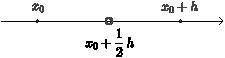
\includegraphics{figures/calculus-rudiments06}
\par\end{center}

dengan mengikuti langkah-langkah berikut. \hasasolution 
\begin{enumerate}
\item Tuliskan $L_{1}(x)$, yaitu bentuk Lagrange dari polinom interpolasi
yang melalui titik-titik
\[
(x_{0},f(x_{0}))\quad\mbox{dan}\quad(x_{1},f(x_{1})).
\]
\item Hitung turunan $L_{1}'(x)$.
\item Substitusikan $x_{0}+\frac{1}{2}h$ untuk $x$ dan $x_{0}+h$ untuk
$x_{1}$ ke dalam rumus yang Anda peroleh pada bagian (b), lalu sederhanakan.
\end{enumerate}
\item Turunkan rumus hampiran untuk turunan pertama pada stensil

\begin{center}
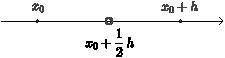
\includegraphics{figures/calculus-rudiments06}
\par\end{center}

dengan mengikuti langkah-langkah berikut.
\begin{enumerate}
\item Tuliskan $L_{1}(x(\theta))=L_{1}(x_{0}+\theta h)$, yaitu bentuk Lagrange
dari polinom interpolasi yang melalui titik-titik
\[
(x_{0},f(x_{0}))\quad\mbox{dan}\quad(x_{0}+h,f(x_{0}+h))
\]
dalam bentuk $\theta$, $h$, dan $x_{0}$.
\item Hitung turunan $\frac{d}{dx}L_{1}(x(\theta))$. Ingat bahwa $x(\theta)=x_{0}+\theta h$,
lalu gunakan aturan rantai.
\item \label{exc:rudiments-4}Substitusikan $\theta=\frac{1}{2}$ ke dalam
rumus yang Anda peroleh pada bagian (b), lalu sederhanakan. \hasananswer 
\end{enumerate}
\item Turunkan rumus hampiran untuk turunan pertama pada stensil

\begin{center}
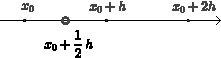
\includegraphics{figures/calculus-rudiments21}
\par\end{center}

 dengan mengikuti langkah-langkah berikut.
\begin{enumerate}
\item Hitung $N_{2}(x)$, yaitu bentuk Newton dari polinom interpolasi yang
melalui titik-titik
\[
(x_{0},f(x_{0})),\ (x_{1},f(x_{1})),\ \mbox{dan}\ (x_{2},f(x_{2})).
\]
\item Hitung turunan $N_{2}'(x)$.
\item \label{exc:rudiments-5}Substitusikan $x_{0}+\frac{1}{2}h$ untuk
$x$, $x_{0}+h$ untuk $x_{1}$, dan $x_{0}+2h$ untuk $x_{2}$ ke
dalam rumus yang Anda peroleh pada bagian (b), lalu sederhanakan. \hasananswer 
\end{enumerate}
\item \label{exc:rudiments-6}Turunkan rumus hampiran untuk turunan kedua
pada stensil

\begin{center}
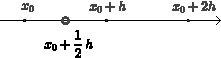
\includegraphics{figures/calculus-rudiments21}
\par\end{center}

dengan mengikuti langkah-langkah berikut. \hasasolution 
\begin{enumerate}
\item Hitung $N_{2}(x(\theta))=N_{2}(x_{0}+\theta h)$, yaitu bentuk Newton
dari polinom interpolasi yang melalui titik-titik
\[
\begin{gathered}(x_{0},f(x_{0})),\ (x_{0}+h,f(x_{0}+h)),\\
\mbox{dan}\ (x_{0}+2h,f(x_{0}+2h))
\end{gathered}
\]
dalam bentuk $\theta$, $h$, dan $x_{0}$.
\item Hitung turunan $\frac{d^{2}}{dx^{2}}N_{2}(x(\theta))$. Ingat bahwa
$x(\theta)=x_{0}+\theta h$, lalu gunakan aturan rantai.
\item Substitusikan $\theta=\frac{1}{2}$ ke dalam rumus yang Anda peroleh
pada bagian (b), lalu sederhanakan.
\end{enumerate}
\item Rumus \ref{eq:centeredDifferenceNaive} dan rumus yang Anda peroleh
dari soal \ref{exc:rudiments} seharusnya berbeda. Namun, keduanya
diturunkan pada stensil yang pada dasarnya sama---dua simpul dengan
titik evaluasi yang berada tepat di tengah keduanya. Hanya label pada
stensil tersebut yang berbeda. Dengan kata lain, keduanya diturunkan
dari geometri yang sama sehingga, dalam arti tertentu, keduanya pasti
sama. Dalam soal \ref{exc:rudiments}, $x_{0}$ memiliki peran yang
sama dengan $x_{0}-h$ dalam \ref{eq:centeredDifferenceNaive}. Selain
itu, dalam soal \ref{exc:rudiments}, jarak dari titik evaluasi ke
masing-masing simpul adalah $\frac{h}{2}$ sedangkan dalam \ref{eq:centeredDifferenceNaive},
jarak tersebut adalah $h$. Lakukan substitusi $x_{0}$ untuk $x_{0}-h$
dalam \ref{eq:centeredDifferenceNaive}. Kemudian substitusikan $\frac{h}{2}$
untuk $h$ pada penyebut \ref{eq:centeredDifferenceNaive}. Dengan
substitusi ini, rumus \ref{eq:centeredDifferenceNaive} seharusnya
sama persis dengan rumus yang Anda peroleh dalam soal \ref{exc:rudiments}.
Dengan kata lain, pelabelan yang berbeda pada suatu stensil menghasilkan
pelabelan yang berbeda pada rumus terkait. Tidak lebih dari itu.
\item \label{exc:rudiments-1}Gunakan rumus \ref{eq:integral7dumb} untuk
menghampiri integral berikut.

\begin{enumerate}
\item \label{exc:rudiments-7}${\displaystyle \int_{-4}^{3}e^{x}dx}$ \hasananswer 
\item ${\displaystyle \int_{-1}^{6}\sin x\,dx}$
\item \label{exc:rudiments-8}${\displaystyle \int_{10}^{17}\frac{1}{x-5}dx}$
 \hasasolution 
\item ${\displaystyle \int_{-3}^{4}\left(x^{5}-4\right)dx}$
\item \label{exc:rudiments-9}${\displaystyle \int_{0}^{1}e^{-x}dx}$ \hasananswer 
\item ${\displaystyle \int_{-\pi/2}^{\pi/2}\cos x\,dx}$
\item \label{exc:rudiments-10}${\displaystyle \int_{1}^{2}\frac{1}{x}dx}$ \hasananswer 
\item ${\displaystyle \int_{4}^{6.1}\left(9-x^{4}\right)dx}$
\end{enumerate}
\item \label{exc:rudiments-11}Untuk setiap integral pada soal \ref{exc:rudiments-1},
(i) hitung integral tersebut secara eksak, dan (ii) hitung galat absolut
pada hampirannya. \haspartwithsolution  \haspartwithanswer 
\item \label{exc:rudiments-2}Misalkan $f(x)=(x-1)^{2}\sin x$. Gunakan
rumus \ref{eq:derivativeDumb} untuk menghampiri $f'(0)$ dengan menggunakan

\begin{enumerate}
\item $h=1$
\item \label{exc:rudiments-12}$h=\frac{1}{2}$ \hasananswer 
\item $h=\frac{1}{4}$
\item $h=\frac{1}{8}$
\end{enumerate}
\item \label{exc:rudiments-13}Hitung galat absolut pada setiap hampiran
dalam soal \ref{exc:rudiments-2}. Apakah galat tersebut mengecil
ketika $h$ mengecil? \haspartwithanswer 
\item \label{exc:rudiments-28}Turunkan rumus hampiran pada stensil

\begin{center}
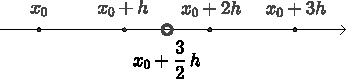
\includegraphics{figures/calculus-rudiments07}
\par\end{center}
\begin{enumerate}
\item untuk nilai fungsi.
\item untuk turunan pertama.
\item untuk turunan kedua.
\item untuk turunan ketiga. Apa yang dapat Anda simpulkan tentang rumus
ini?
\end{enumerate}
\item Polinom $p(x)=3x^{4}-2x^{2}+x-7$ adalah polinom interpolasi untuk
$f$. Gunakan $p$ untuk mengaproksimasi

\begin{enumerate}
\item $f(1)$
\item \label{exc:rudiments-14}$f(2)$ \hasananswer 
\item $f'(1)$
\item \label{exc:rudiments-15}$f'(2)$ \hasasolution 
\item ${\displaystyle \int_{0}^{1}f(x)dx}$
\item \label{exc:rudiments-16}${\displaystyle \int_{0}^{2}f(x)dx}$ \hasananswer 
\end{enumerate}
\item Polinom $q(x)=-7x^{4}+3x^{2}-x+4$ adalah polinom interpolasi untuk
$g$. Gunakan $q$ untuk mengaproksimasi

\begin{enumerate}
\item \label{exc:rudiments-17}$g(1)$ \hasananswer 
\item $g(2)$
\item \label{exc:rudiments-18}$g'(1)$ \hasananswer 
\item $g'(2)$
\item \label{exc:rudiments-19}${\displaystyle \int_{0}^{1}g(x)dx}$ \hasasolution 
\item ${\displaystyle \int_{0}^{2}g(x)dx}$
\end{enumerate}
\item Gunakan \ref{eq:p2relativeDerivative} untuk menentukan rumus turunan
pertama pada stensil

\begin{enumerate}
\item \raisepic{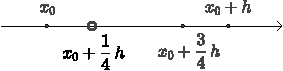
\includegraphics{figures/calculus-rudiments08}}\medskip 
\item \label{exc:rudiments-20}\raisepic{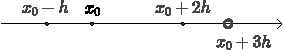
\includegraphics{figures/calculus-rudiments10}}\medskip  \hasananswer 
\item \raisepic{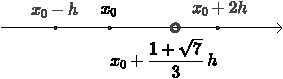
\includegraphics{figures/calculus-rudiments11}}\medskip 
\item \label{exc:rudiments-21}\raisepic{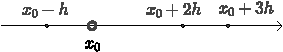
\includegraphics{figures/calculus-rudiments09}}\medskip  \hasasolution 
\item \raisepic{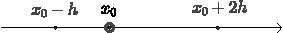
\includegraphics{figures/calculus-rudiments12}}\medskip 
\item \label{exc:rudiments-22}\raisepic{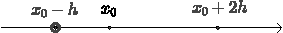
\includegraphics{figures/calculus-rudiments15}}\medskip  \hasananswer 
\item \raisepic{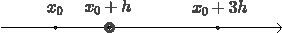
\includegraphics{figures/calculus-rudiments13}}\medskip 
\item \label{exc:rudiments-23}\raisepic{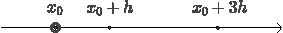
\includegraphics{figures/calculus-rudiments14}} \hasananswer 
\end{enumerate}
\item \label{exc:rudiments-3}Tentukan rumus hampiran umum untuk integral
dengan menggunakan dua simpul melalui langkah-langkah berikut.

\begin{enumerate}
\item Tuliskan polinom interpolasi linear dengan simpul-simpul $x_{0}+\theta_{2}h$
dan $x_{0}+\theta_{3}h$.
\item Integralkan polinom tersebut pada interval $[x_{0}+\theta_{0}h,x_{0}+\theta_{1}h]$.
\item \label{exc:rudiments-24}Sederhanakan. \hasananswer 
\end{enumerate}
\item Gunakan rumus hampiran umum yang Anda turunkan dalam soal \ref{exc:rudiments-3}
untuk memperoleh rumus hampiran pada stensil.

\begin{enumerate}
\item \label{exc:rudiments-25}\raisepic{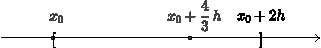
\includegraphics{figures/calculus-rudiments16}}\medskip  \hasananswer 
\item \raisepic{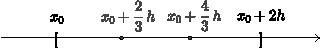
\includegraphics{figures/calculus-rudiments17}}\medskip 
\item \label{exc:rudiments-26}\raisepic{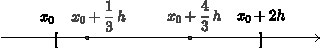
\includegraphics{figures/calculus-rudiments18}}\medskip  \hasasolution 
\item \raisepic{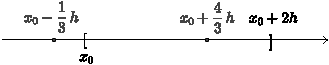
\includegraphics{figures/calculus-rudiments19}}\medskip 
\item \label{exc:rudiments-27}\raisepic{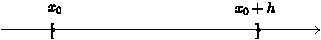
\includegraphics{figures/calculus-rudiments20}} \hasananswer 
\end{enumerate}
\item Rumus umum tiga titik untuk turunan pertama yang menggunakan $f(x_{0})$,
$f(x_{0}+\alpha h)$, dan $f(x_{0}+2h)$, dengan $\alpha\neq0$ dan
$\alpha\neq2$, diberikan oleh
\begin{eqnarray*}
f'(x_{0}) & = & \frac{1}{2h}\left[-\frac{2+\alpha}{\alpha}f(x_{0})\right.\\
 &  & \qquad+\frac{4}{\alpha(2-\alpha)}f(x_{0}+\alpha h)\\
 &  & \qquad\left.-\frac{\alpha}{2-\alpha}f(x_{0}+2h)\right]+O(h^{2})
\end{eqnarray*}

Gunakan ekspansi Taylor dari $f(x_{0}+\alpha h)$ dan $f(x_{0}+2h)$
untuk menurunkan rumus yang diberikan.
\end{enumerate}
\noindent\finishexercises 

\subsection{Jawaban}
\begin{description}
\item [{\textmd{$\int_{x_{0}+2.5h}^{x_{0}+6h}f(x)dx$:\label{ans:integralFormula1}}}] 
\[
\begin{gathered}\frac{1/35}{138240}\left[42056(1.971614474758557)+201831(1.981091507449763)\right.\\
+63357(1.993574976724822)+195902(2.009751835391139)\\
-28518(2.030278824314539)+10731(2.055494116570853)\\
\left.-1519(2.084603181618954)\right]
\end{gathered}
\]
 
\item [{$\int_{x_{0}-h}^{x_{0}+6h}f(x)dx$:\label{ans:integralFormula2}}] 
\[
\begin{gathered}\frac{1/7}{8640}\left[5257(1.96122825291126)-5880(1.965674866641883)\right.\\
+59829(1.960870620285721)-81536(1.941460911122824)\\
+102459(1.923339403354019)-50568(1.951091775564697)\\
\left.+30919(1.9498808918992)\right]
\end{gathered}
\]
\end{description}

